{\kaishu 9.7-9.11热学}

\lsn{1}默写与理想气体相关的公式：
\begin{table}[htbp]
  \begin{tabular}{r p{4cm}|rp{4cm}}
    \toprule
    &公式&&公式\\
    \hline
    气体压强&&液体压强&\\
    \hline
    理想气体方程&&克拉珀龙方程&\\
    \hline
    玻意耳定律&&查理定律&\\
    \hline
    盖吕萨克定律&&密度方程&\\
    \hline
    混合气体方程&\multicolumn{3}{c}{}\\
    \bottomrule
  \end{tabular}
\end{table}

\lsn{2}默写热力学三定律：
\vspace*{4cm}

\lsn{3}画出分子间作用力和分子势能的图像：
\vspace*{4cm}

\lsn{4}分析扩散和布朗运动的异同：
\vspace*{4cm}

\lsn{5}已知\ce{Cu}的密度为\(\rho\)，摩尔质量为\(M\)，阿伏加德罗常数为\(N_A\)，求\ce{Cu}的原子直径\(d\)。

\newpage

\lsn{6}证明：缓慢加热气缸中的气体，活塞缓慢移动，该变化为等压变化。
\vspace*{3cm}

\lsn{7}大气压强均为\(p_0\)，写出下图中气体压强：

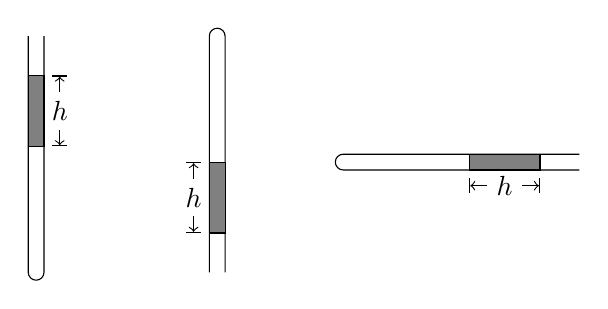
\begin{tikzpicture}
    
	\begin{scope}[]
		\draw[|<->|] (.4,1.6)--node[fill=white]{\(h\)}(.4,2.5);
		\draw (0,3)--(0,0) arc(-180:0:.1)--(.2,3);
		\draw[fill=gray] (0,1.6) rectangle(.2,2.5);
	\end{scope}
    \begin{scope}[xshift=2.5cm,yshift=3cm,rotate=180]
		\draw[|<->|] (.4,1.6)--node[fill=white]{\(h\)}(.4,2.5);
		\draw (0,3)--(0,0) arc(-180:0:.1)--(.2,3);
		\draw[fill=gray] (0,1.6) rectangle(.2,2.5);
	\end{scope}
    \begin{scope}[xshift=4cm,yshift=1.5cm,rotate=-90]
        \draw[|<->|] (.4,1.6)--node[fill=white]{\(h\)}(.4,2.5);
		\draw (0,3)--(0,0) arc(-180:0:.1)--(.2,3);
		\draw[fill=gray] (0,1.6) rectangle(.2,2.5);
	\end{scope}
\end{tikzpicture}
\hspace*{3em}
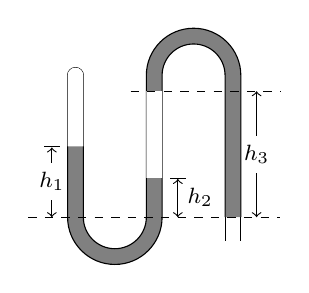
\begin{tikzpicture}[font=\footnotesize]
    \draw[|<->] (-.2,.9)--node[fill=white]{\(h_1\)}(-.2,0);
    \draw[|<->] (1.4,.5)--node[right]{\(h_2\)}(1.4,0);
    \draw[<->] (2.4,1.6)--node[fill=white]{\(h_3\)}(2.4,0);
    \draw[fill=gray] (2,0)--(2,1.8) arc(0:180:.4)--(1.2,0) arc(0:-180:.6)--(0,1.8) arc(180:0:.1)--(.2,0) arc(-180:0:.4)--(1,1.8) arc(180:0:.6)--(2.2,0);
    \fill[white] (0,.9)--(0,1.8)arc(180:0:.1)--(.2,.9)--(0,.9) (1,.5) rectangle(1.2,1.6);
    \draw (2,0)--(2,-.3) (2.2,0)--(2.2,-.3);
    \draw[dashed] (-.5,0)--(2.7,0) (.8,1.6)--(2.7,1.6);
\end{tikzpicture}
\vspace*{1.5cm}

\lsn{8}第一类永动机和第二类永动机为什么不可能存在？
\vspace*{2.5cm}

\lsn{9}如下图所示，将粗细不同的玻璃管插入水和水银中，试画出试管中的液面

\begin{tikzpicture}[font=\footnotesize]
    \draw[fill=gray!30] (0,0) rectangle(4,1.5);
    \draw[very thick] (0,3)--(0,0)--(4,0)--(4,3);
    \draw[fill=white,draw=white] (1.4,.5) rectangle(1.7,1.6) (2.5,.5) rectangle(2.65,1.6);
    \foreach \x in {1.4,1.7,2.5,2.65}
        \draw[very thin] (\x,.5)--(\x,2.8);
    \node at(3.5,.4){水};
    \begin{scope}[xshift=6cm]
        \draw[fill=gray!30] (0,0) rectangle(4,1.5);
        \draw[very thick] (0,3)--(0,0)--(4,0)--(4,3);
        \draw[fill=white,draw=white] (1.4,.5) rectangle(1.7,1.6) (2.5,.5) rectangle(2.65,1.6);
        \foreach \x in {1.4,1.7,2.5,2.65}
            \draw[very thin] (\x,.5)--(\x,2.8);
        \node at(3.5,.4){水银};
    \end{scope}
\end{tikzpicture}

\lsn{10}一只轮胎容积为\(V=\) \,\qty{10}{L}，已装有\(p_1 =\) \,\qty{1}{atm}的空气。现用打气筒给打气，已知打气筒的容积为\(V_0 =\) \,\qty{1}{L}，要使胎内气体压强达到\(p_2 =\) \,\qty{2.5}{atm}，应至少打多少次气？(设打气过程中轮胎容积及气体温度维持不变，大气压强\(p_0 =\) \,\qty{1}{atm})
\vspace*{2cm}

\lsn{11}在测油酸分子直径的实验中，如果使用长时间放置的酒精油酸溶液，测得的油酸分子直径会偏大还是偏小？为什么？

\newpage
\lsn{12}质量不变的理想气体经历\(a \to b \to c \to a\)的循环过程，其中\(a\to b\)是等温膨胀过程，\(b\to c\) 是等容过程，\(c\to a\)是等压过程，分别在\(p - V\)、\(p - T\)、\(V - T\)图像中画出该循环过程，并分析各个过程的\(\Delta U\)、\(W\)、\(Q\) 以及整个循环过程是吸热还是放热。

\begin{tikzpicture}[font=\footnotesize,>=latex]
    \draw[blue,->] (0,0)node[below left]{\(O\)}--(4,0) node[right]{\(V\)};
    \draw[blue,->] (0,0)--(0,3) node[above]{\(p\)};
\end{tikzpicture}
\vspace*{1cm}

\begin{tikzpicture}[font=\footnotesize,>=latex]
    \draw[blue,->] (0,0)node[below left]{\(O\)}--(4,0) node[right]{\(T\)};
    \draw[blue,->] (0,0)--(0,3) node[above]{\(p\)};
\end{tikzpicture}
\vspace*{1cm}

\begin{tikzpicture}[font=\footnotesize,>=latex]
    \draw[blue,->] (0,0)node[below left]{\(O\)}--(4,0) node[right]{\(T\)};
    \draw[blue,->] (0,0)--(0,3) node[above]{\(V\)};
\end{tikzpicture}